\setcounter{chapter}{2}

\chapter{函数极限与连续}

\section{函数极限的概念与性质}

函数极限是我们后续定义导数、积分的概念的基础,因此可以说函数极限的理论也是整个
微积分学的基础。

\subsection{函数极限的概念}

不同于数列极限只有单一的$n\to\infty$一种(自变量的变化)趋势,
{\bf 函数极限共有六种可能的(自变量变化)趋势},分为两大类:

\begin{itemize}
  \setlength{\itemindent}{1cm}
  \item 趋于无穷
  $$x\to\infty,\quad x\to+\infty,\quad x\to-\infty$$
  \item 趋于有限值
  $$x\to x_0,\quad x\to x_0^+,\quad x\to x_0^-$$
\end{itemize}

{\bf 思考:} $\limn f(n)=A\Leftrightarrow\limx{+\infty}f(x)=A$?

{\bf 答}:显然,{\b$\limx{+\infty}f(x)=A$显然可以推出$\limn f(n)=A$,但反之不然},
\ps{$f(n)$的值域是$f(x)$值域的子集}

例如:$y=\sin\pi x$当$x\to+\infty$时不收敛,但$\limn\sin n\pi=0$。

\subsubsection{【趋于无穷时的函数极限】}

{\bf 定义3.1.1}
\ps{\b 和$\limn a_n=a$的定义做类比,理解(1),然后推广到(2),(3)}
\begin{enumerate}[(1)]
  \setlength{\itemindent}{1cm}
  \item $\limx{+\infty}f(x)=A\Leftrightarrow\forall \e>0,\exists X,\forall
  x>X,|f(x)-A|<\e$
  \item $\limx{-\infty}f(x)=A\Leftrightarrow\forall \e>0,\exists X,\forall
  x<X,|f(x)-A|<\e$
  \item $\limx{\infty}f(x)=A\Leftrightarrow\forall \e>0,\exists X,\forall
  |x|>X,|f(x)-A|<\e$
\end{enumerate}

{\bf 例:}证明$\limx{+\infty}\df1{\sqrt x}=0$.

{\bf 注:}不等式右端的$\e$可以改写为$C\e$,其中$C>0$为常数

{\bf 注:}{\b 趋于无穷的函数极限存在,意味着函数存在{\it 水平渐近线}},
且水平渐近线最多可以有两条,例如:$y=\arctan x$

% \begin{center}
% 	\resizebox{!}{4cm}{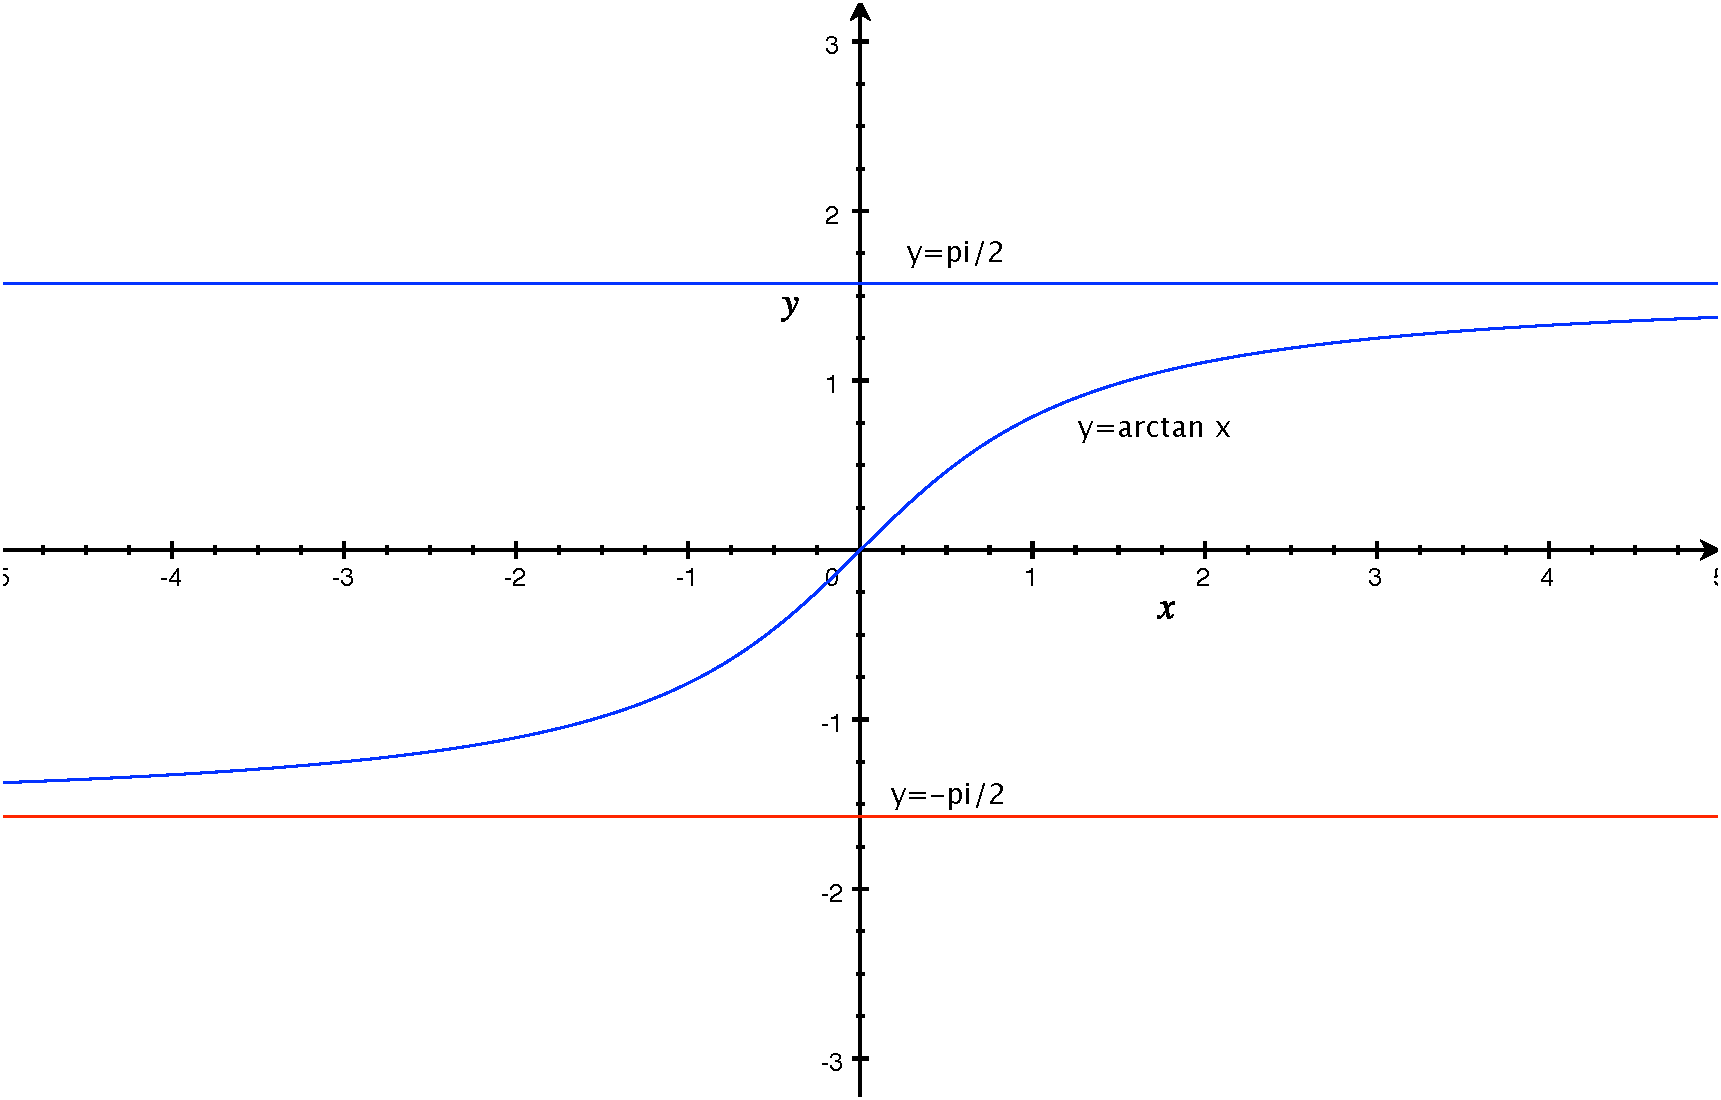
\includegraphics{./images/ch3/arctan.pdf}}
% \end{center}

\begin{center}
	\begin{overpic}[scale=0.3]{./images/ch3/arctan.pdf}
		\put(0,10){\b $\limx{-\infty}\arctan x=-\df{\pi}2$}
		\put(65,53){\b $\limx{+\infty}\arctan x=\df{\pi}2$}
	\end{overpic}
\end{center}

\subsubsection{【趋于有限值时的函数极限】}

{\bf 定义3.1.2}
\begin{enumerate}[(1)]
  \setlength{\itemindent}{1cm}
  \item $\limx{x_0}f(x)=A\Leftrightarrow\forall \e>0,\exists\delta>0,\forall
  x\in U_0(x_0,\delta),|f(x)-A|<\e$
  \item $\limx{x_0^+}f(x)=A\Leftrightarrow\forall \e>0,\exists\delta>0,\forall
  x\in(x_0,x_0+\delta),|f(x)-A|<\e$
  \item $\limx{x_0^-}f(x)=A\Leftrightarrow\forall \e>0,\exists\delta>0,\forall
  x\in(x_0-\delta,x_0),|f(x)-A|<\e$
\end{enumerate}

{\bf 例}(习题3.1-1)根据图形判断极限的存在性
\begin{center}
	\resizebox{!}{4cm}{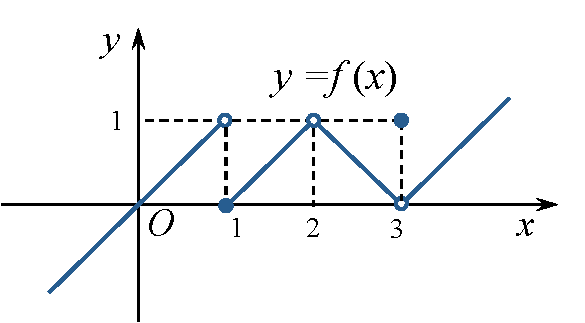
\includegraphics{./images/ch3/limxf.pdf}}
\end{center}
\begin{enumerate}[(1)]
  \setlength{\itemindent}{1cm}
  \item $\limx{1}f(x)$\underline{不存在}
  \item $\limx{2}f(x)$\underline{$=1$}
  \item $\limx{1}f(x)$\underline{$=0$}
\end{enumerate}

{\bf 思考:}
\begin{itemize}
  \setlength{\itemindent}{1cm}
  \item 为什么在定义中要求$0<|x-x_0|<\delta$,而不是$|x-x_0|<\delta$?
  {\it (因为极限表示一种趋势,与函数在该点处的取值无关)}
  \item $f(x_0+0),f(x_0-0)$与$f(x_0)$是何关系?
  {\it(前两者分别表示左右极限,最后一个是函数值,三者相互无关)}
\end{itemize}

{\bf 例:}证明
\begin{enumerate}[(1)]
  \setlength{\itemindent}{1cm}
  \item $\limx{x_0}\sin x=\sin x_0$
  \item $\limx{1}x^2=1$
%   \item $\limx{1}\df1x=1$
\end{enumerate}

{\bf 证:}(1)对任意$\e>0$,令{\b$\delta=\e$},则当$0<|x-x_0|<\delta$时,有
$$|\sin x-\sin x_0|=2\left|\cos\df{x+x_0}2\right|
\left|\sin\df{x-x_0}2\right|\leq|x-x_0|<\delta=\e,$$
由函数极限定义,即证。

(2) 对任意$\e>0$,令{\b$\delta=\min\left\{\df12,\e\right\}$},
\ps{令$\delta\leq\df12$,作用在于使得$|x+1|$有界}
则当$0<|x-1|<\delta$时,有
$$|x^2-1|=|(x+1)(x-1)|<\df32\cdot\delta<\df32\e,$$
由函数极限定义,即证。

\begin{shaded}
	{\bf 【函数极限的反面说法】}
	
	\begin{itemize}
	  \item 当$x\to x_0$时$f(x)$不以$A$为极限 
	    $$\exists\e_0>0,\forall\delta>0, \exists x^*\in
	    U_0(x_0,\delta),|f(x^*)-A|\geq\e_0$$ 
	  \item 当$x\to x_0$时$f(x)$无极限
		$$\forall A\in\mathbb{R},\exists\e_0>0,\forall\delta>0, \exists x^*\in
	    U_0(x_0,\delta),|f(x^*)-A|\geq\e_0$$ 
	\end{itemize}
	
	{\bf 例:}证明:Dirichlet函数在任意点处无极限。
\end{shaded}

\subsection{函数极限的基本性质}

\subsubsection{【唯一性】}

{\bf 定理3.1.2:}函数极限若存在,必唯一。

\subsubsection{【有界性】}

{\bf 定理3.1.3:}
\begin{enumerate}[(1)]
  \setlength{\itemindent}{1cm}
  \item 若$\limx{+\infty}f(x)=A$,则$f(x)$当$x$充分大时有界
  \item 若$\limx{x_0}f(x)=A$,则$f(x)$在$x_0$的某去心领域内有界
\end{enumerate}

{\bf 注意:}函数极限有界性和数列极限有界性的叙述存在的差异:
{\it\b 数列收敛则数列整体有界,函数收敛只能说明在趋近的过程中有界!}
\ps{数列极限中的数列整体有界,
是由数列自身的“稀疏”特性所决定的}

\subsubsection{【保号性】}

{\bf 定理3.1.4:}
\begin{enumerate}[(1)]
  \setlength{\itemindent}{1cm}
  \item 若$\limx{+\infty}f(x)=A>0$,则当$x$充分大时,$f(x)>0$
  \item 若$\limx{x_0}f(x)=A>0$,则在$x_0$的某去心领域内,$f(x)>0$
\end{enumerate}

{\bf 课堂思考:}
\begin{enumerate}[(1)]
  \setlength{\itemindent}{1cm}
  \item 若$x\to x_0$时,$f(x)$有极限,$g(x)$无极限,则当$x\to x_0$时,以下哪些函数必无极限:
  $$f(x)g(x),\quad [g(x)]^2,\df{g(x)}{f(x)}, f(x)+g(x)$$ 
  \item 若$\limx{x_0}g(x)=A,\lim\limits_{u\to A}f(u)=B$,是否必有
  $$\limx{x_0}f[g(x)]=B\;?$$
  \item 若$\limx{x_0}f(x)g(x)=0$,则当$x\to
  x_0$时, $f(x),$ $g(x)$之一必趋于$0$ ({$\times$})
\end{enumerate}

{\bf 例:}设$\limx{x_0}f(x)=A$,用定义证明:$\limx{x_0}[f(x)]^3=A^3$

{\bf 证:}对任意$\e>0$,由$\limx{x_0}f(x)=A$,存在$\delta>0$,对任意
$0<|x-x_0|<\delta$,有
$$|f(x)-A|<\e.$$
不妨设$\e<1$,由上式可知$0<|x-x_0|<\delta$时,有$|f(x)|<|A|+1$。

综上,记$C=(|A|+1)^2+(|A|+1)|A|+A^2$,则当$0<|x-x_0|<\delta$时,总有
\begin{align}
	|f^3(x)-A^3|&=|f(x)-A||f^2(x)+f(x)A+A^2|\notag\\
	&\leq |f(x)-A|[|f^2(x)|+|f(x)||A|+A^2]\notag\\
	&<\e[(|A|+1)^2+(|A|+1)|A|+A^2]=C\e\notag,
\end{align}
有极限的定义,即证。

\section{函数极限的判敛}

\subsection{四则运算}

{\bf 定理3.2.1:}若函数极限存在,则极限运算可以和四则运算交换次序。

{\bf 注:}把握两点
\begin{itemize}
  \setlength{\itemindent}{1cm}
  \item 有限次四则运算
  \item 可以推广到初等函数
\end{itemize}

\subsection{复合函数的极限}

{\bf 定理3.2.2:}设有复合函数$y=f[g(x)]$,其中\ps{与子数列的收敛性质作对比}
$$\limx{x_0}g(x)=u_0,\quad\lim\limits_{u\to u_0}f(u)=A,$$
在$x_0$附近$g(x)\ne u_0$,则
$$\limx{x_0}f[g(x)]=A.$$

{\bf 注:}
\begin{itemize}
  \setlength{\itemindent}{1cm}
  \item 直观理解:若相关极限都存在,则极限运算可以和函数运算交换次序
  \item {\b 为什么要求“在$x_0$附近$g(x)\ne u_0$”?}
  
  {\it 答:因为$f(x)$可能在$x_0$处的定义与极限值无关,例如:
  $$f(x)=\left\{\begin{array}{ll}
  1,&x\ne0\\0,&x=0
  \end{array}\right.$$
  $g(x)\equiv 0$,则$f(g(x))\equiv0$,从而$\limx{0}f(g(x))=0$,
  而不是如定理所述$\limx{0}f(g(x))=1$}
  \item 可以类似地推广到$x\to\infty$的情形
\end{itemize}

\subsection{函数极限与数列极限的关系}

{\bf 定理3.2.3}(Hiene定理)$\limx{\Delta}f(x)=A\Leftrightarrow
$若数列$\{x_n\}$满足:$x_n\to \Delta(n\to$ $\infty)$,则
$$\limn f(x_n)=A$$

\begin{itemize}
  \setlength{\itemindent}{1cm}
  \item 以上$\Delta$对应于函数极限的六种不同趋势 
  \item {\bf 用途一:}证明极限不存在性
  \item {\bf 用途二:}利用函数极限计算对应的数列极限
\end{itemize}

{\bf 教材3.2.2节-例8:}{\b 证明:$f(x)=\sin\df 1x$当$x\to 0$时无极限。}

{\bf 证}:令
$$x^{(1)}_n=\df1{n\pi},\quad
x^{(2)}_n=\df1{2n\pi+\df{\pi}2},\quad n\in\mathbb{Z}_+$$ 
显然,$\limn x^{(1)}_n=\limn x^{(2)}_n=0$,且
$$f(x^{(1)}_n)\equiv0,\quad f(x^{(2)}_n)\equiv1,$$
进而
$$\limn f(x^{(1)}_n)=0\ne1=\limn f(x^{(2)}_n),$$
由Henie定理,即知极限不存在。

\begin{center}
	\resizebox{!}{5cm}{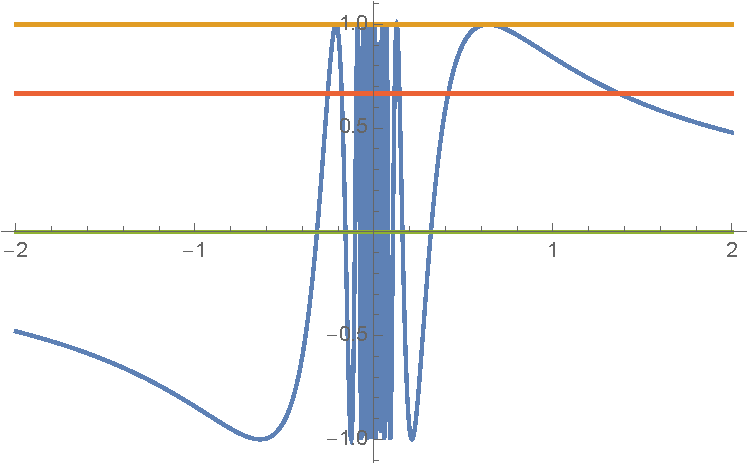
\includegraphics{./images/ch3/sin1x.pdf}}
	
	{\it 以上所取的$x^{(1)}_n$和$x^{(2)}_n$分别取自图上绿色和黄色水平线与
	函数$\sin\df1x$的交点,事实上,对于任意的$a\in[-1,1]$(红色水平线),
	都可以取得类似的点列,用于构造证明所需的收敛到不同值得函数值数列,请思考以下如何写
	出其表达式?
	$$x^{(a)}_n=\df1{2n\pi+\arcsin a},\quad n\in\mathbb{Z}_+$$}
\end{center}

{\bf 例}(习题3.2-7)证明Dirichlet函数在任意点处无极限。

\begin{shaded}
	{\bf 命题:}对任意$x_0\in\mathbb{R}$,都存在这样的两个数列
	$\{x_n^{(1)}\}$和$\{x_n^{(2)}\}$,满足
	$$x_n^{(1)}\in\mathbb{Q},\;x_n^{(2)}\notin\mathbb{Q}\;(n\in\mathbb{Z}_+),$$
	且
	$$\limn x_n^{(1)}=\limn x_n^{(2)}=x_0.$$
	
	{\bf 思考:}试给出$\{x_n^{(1)}\}$和$\{x_n^{(2)}\}$的通项表达式。
	
	{\bf 参考答案:}1)若$x_0\in\mathbb{Q}$,可令
	$$x_n^{(1)}=x_0+\df1n,\quad
	x_n^{(2)}=x_0+\df{\sqrt2}n,\;(n\in\mathbb{Z}_+)$$
	2)若$x_0\notin\mathbb{Q}$,可令
	$$x_n^{(1)}=[x_0]+x_0\mbox{\it 小数部分的前}n\mbox{\it 位},
	\;(n\in\mathbb{Z}_+)$$
	例如$x_0=\pi=3.1415926\ldots$,则
	$$x_1^{(1)}=3.1,\;x_2^{(1)}=3.14,\;x_3^{(1)}=3.141,\;
	x_4^{(1)}=3.1415,\;\ldots$$
	另,
	$$x_n^{(2)}=x_0+\df1n,\;(n\in\mathbb{Z}_+)$$
\end{shaded}

{\bf 例:}设在$(0,+\infty)$上,恒有$f(x^2)=f(x)$,且
$$\limx{0^+}f(x)=\limx{+\infty}f(x)=f(1)$$
证明:$f(x)=f(1)\,(x\in(0,+\infty))$

\subsection{夹逼定理}

{\bf 定理3.2.5:}设在$x_0$的某邻域内,恒有
$$\varphi(x)\leq f(x)\leq\psi(x), $$
且$\limx{x_0}\varphi(x)=\limx{x_0}\psi(x)=A$,则
$$\limx{x_0}f(x)=A.$$

{\bf 教材3.2.3节-例9}(重要极限一)证明:
$$\limx{\infty}\left(1+\df 1x\right)^x=e$$

[思路]:利用数列极限$\limn\left(1+\df1n\right)^n=e$,构造夹逼所需的函数
$$\left(1+\df1{[x]+1}\right)^{[x]}<\left(1+\df1x\right)^x
<\left(1+\df1{[x]}\right)^{[x]+1},$$
然后利用函数极限的运算性质,证明不等式两端函数当$x\to+\infty$时,极限均为$e$。

$x\to-\infty$的结果利用极限运算的性质易证。

\begin{shaded}
{\bf 例}(另一种证明思路)令$f_u=x^ue^{-x}(x\geq 0)$,对于确定的$u$,证明:
\begin{enumerate}[(1)]
  \setlength{\itemindent}{1cm}
  \item $f_u(x)$在$x=u$处取最大值;
  \item 由$f_u(x)>f_u(u+1)$和$f_{u+1}(u+1)>f_u(u)$推出
  $$\left(\df{u+1}u\right)^u<e<\left(\df{u+1}u\right)^{u+1}$$
  \item $\df u{u+1}e<\left(\df{u+1}u\right)^u<e$,由此推出
  $$\limx{+\infty}\left(1+\df 1u\right)^u=e$$
\end{enumerate}
\end{shaded}

{\b{\bf 例:}{\it 这些都是重要极限的应用,须牢记有关结果!!!}
\begin{enumerate}[(1)]
  \setlength{\itemindent}{1cm}
  \item $\limx{0}(1+x)^{1/x}$ 
  \item $\limx 0(1+\sin x)^{1/\sin x}$ 
  \item $\limx 0\df{\ln(1+ax)}{x}$
  \item $\limx 0\df{e^{ax}-1}{x}$ 
  \item $\limx 0\df{a^x-1}{x}(a>0)$ 
  \item $\limn n(\sqrt[n]{a}-1) (a>0)$ 
\end{enumerate}}

{\bf 教材3.2.3节-例11}(重要极限二)证明:
$$\limx{0}\df {\sin x}x=1$$

{[提示]}:
\begin{center}
	\resizebox{!}{5cm}{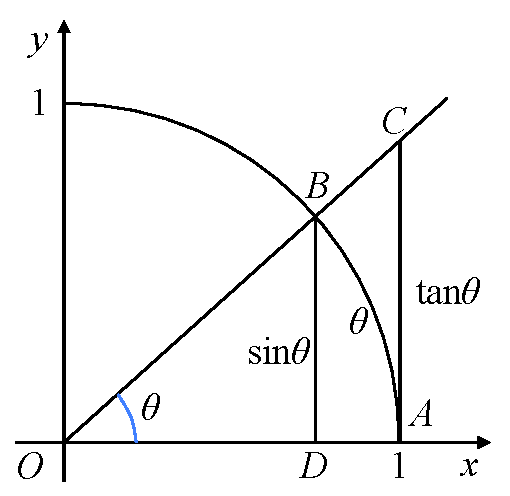
\includegraphics{./images/ch3/xsintan.pdf}}
\end{center}

如图,显然弧$AB$的长度大于直线$BD$,即$\sin\theta<\theta$;又扇形$ABO$的面积$\df12\theta$
小于三角形$ACO$的面积$\df12\tan\theta$,从而$\theta<\tan\theta$

{\b{\bf 例:}{\it 牢记!!!}
\begin{enumerate}[(1)]
  \setlength{\itemindent}{1cm}
  \item $\limx{0}\df{\sin\sin x}{\sin x}$ 
  \item $\limx 0\df{1-\cos x}{x^2}$ 
  \item $\limx 0\df{\sin mx}{\sin nx}(n\ne 0)$
  \item $\limx 0\df{\tan x}{x}$
  \item $\limx a\df{\sin x-\sin a}{x-a}$
\end{enumerate}}

{\bf 例:}设$f(x)=\sum\limits_{i=1}^na_i\sin
ix$,其中$a_i(i=1,2,\ldots,n)$为常数,且对任意$x\in\mathbb{R}$, $|f(x)|\leq |\sin x|$,证明:
$$\left|a_1+2a_2+\ldots+na_n\right|\leq 1$$

[提示]:{\it 极限运算可以和绝对值运算交换次序!}

\section{无穷大、无穷小和函数的渐近线}

在求解(函数)极限的问题中,分子分母同时趋于零
\ps{所谓不定是相对诸如有界量乘以无穷小(趋于零)、有界量除以无穷大一类容易确定的形式而言的}
(例如:$\limx{0}\df{\cos
x-\cos2x}{x^2}$),或者一个趋于零的函数和一个趋于无穷的函数的乘积(例如:$\limx{+\infty}x^2e^-x$)
的极限通常是较难求解的,这类问题我们称之为“$\df00$”和“$0\cdot\infty$” 型的{\it 不定式(极限)}!


{\bf 思考:}除了“$\df00$”和“$0\cdot\infty$”型的不定式,还可能有其他形式的不定式吗?

{\bf 答:}有,型如:“$\df{\infty}{\infty}$”、“$1^{\infty}$”、“$0^0$”,例如:
$\limx{+\infty}\df{\ln x}{x}$,$\limx{\infty}\left(1+\df1{x}\right)^{\sin
x}$,$\limx{0}x^{2x}$

\subsection{无穷大和无穷小}

{\bf 定义3.3.1:}$f(x)$是$x\to\Delta$时的无穷小$\Leftrightarrow\limx{\Delta}f(x)=0$

{\bf 注:}$\Delta$可任意代表$\infty,\;+\infty,\;-\infty,\;x_0,\;x_0^+,\;x_0^-$之一

{\bf 定理3.3.1-3.3.2}(无穷小的性质)
\begin{enumerate}[(1)]
  \setlength{\itemindent}{1cm}
  \item $\limx{\Delta}f(x)=A\in\mathbb{R}\Leftrightarrow
  f(x)-A$是$x\to\Delta$时的无穷小
  \item $x\to\Delta$时的有界函数与无穷小之积仍为$x\to\Delta$时的无穷小
  \item $x\to\Delta$时的有限个无穷小之和(积)仍为$x\to\Delta$时的无穷小
\end{enumerate}

{\bf 定义3.3.2:}$f(x)$是$x\to\Delta$时的无穷大$\Leftrightarrow\limx{\Delta}\df 1{f(x)}=0$,
可记为:
$$\limx{\Delta}f(x)=\pm\infty$$

{\bf 注:}{\b 无穷大有正负之分!!}

{\bf 【渐近线】}\ps{具体内容请阅读教材自学!}

$x\to x_0$时的无穷大意味着存在{\it 铅直渐近线};$x\to\pm\infty$时的无穷大
{\it 可能}意味着存在{\it 斜渐近线},例如:若$y=f(x)$当$x\to+\infty$时的
存在斜渐近线$y=kx+b$,则
$$k=\limx{+\infty}\df{f(x)}x,\quad b=\limx{+\infty}[f(x)-kx].$$
注意,{\b $x\to\pm\infty$时的斜渐近线可能是不同的!}例如:$y=x\arctan x$趋于
$x\to\pm\infty$时的斜渐近线分别为$y=\pm\df{\pi}2x$.

% {\bf P129-例4:}证明:$x+\sin x$是$x\to\infty$时的无穷大

{\bf 定理3.3.3:}在$x\to\Delta$的同一过程中:
\begin{enumerate}[(1)]
  \setlength{\itemindent}{1cm}
  \item 有界函数与无穷大之和仍为无穷大
  \item 有限个无穷大之乘积仍为无穷大({\it 但可能反号})
\end{enumerate}

{\bf 例:}证明:$f(x)=a_0x^n+a_1x^{n-1}+\ldots+a_n(n\in\mathbb{N})$
是$x\to\infty$时的无穷大,其中:$a_0,a_1,\ldots,a_n\in\mathbb{R},a_0\ne 0$

\begin{shaded}
	{\bf 无穷大之间的比较!}
	
	当$x\to+\infty$时,存在如下的大小关系:设$a>0$,
	$$\ln x<<x^a<<e^x<<\Gamma(x)<<x^x$$
	其中$\Gamma-$函数定义为$\Gamma(x)=\dint_0^{+\infty}t^{x-1}e^{-t}\d t$,
	满足$\Gamma(n)=(n-1)!,\;(n\in\mathbb{Z}_+)$
\end{shaded}

\subsection{无穷小的比较}

{\bf 定义3.3.3:}设$y_1,y_2$均为$x\to\Delta$时的无穷小,
$\limx{\Delta}\df{y_1}{y_2}=A$为常数
\begin{enumerate}[(1)]
  \setlength{\itemindent}{1cm}
  \item $A=0$,称$y_1$为$y_2$当$x\to\Delta$时的{\it 高阶(高级)无穷小},记为:
  \ps{\b 等式中出现无穷小符号$\circ$或$\mathrm{O}$时,等号的含义,准确地
  解释应该是指左侧函数为右侧符号所标识的函数之一!}
  $$y_1=\circ( y_2)\;\;(x\to\Delta)$$
  \begin{itemize}
    \item {\it 无穷小}可记为:
    $$y_1=\circ(1)\;\;(x\to\Delta)$$
  \end{itemize}
  \item $A\ne 0$,称$y_1$为$y_2$当$x\to\Delta$时的{\it 同阶(同级)无穷小},记为:
  $$y_1=\mathrm{O}( y_2)\;\;(x\to\Delta)$$
  \item $A=1$,称$y_1$为$y_2$当$x\to\Delta$时的{\it 等价无穷小},记为:
  $$y_1\sim y_2\;\;(x\to\Delta)$$
\end{enumerate}

{\bf 注意:}{\it\b 所有的无穷小都必须是和某个$x\to\Delta$相关的,因此讨论
无穷小性质或者对其进行计算、推导时,必须说明是在怎样的$x$变化趋势之中!!!}

\begin{shaded}
	{\bf 【高阶无穷小的推导关系】}
	对包含有无穷小符号的表达式进行推导,不可避免地会涉及一些化简、合并运算,以下是一些常用
	的化简形式,以$x\to 0$时的无穷小为例:
	\begin{enumerate}[(1)]
  	  \setlength{\itemindent}{1cm}
  	  \item $C\cdot\circ(x^n)=\leadsto\circ(x^n)\;(C\in\mathbb{R}\mbox{为常数})$
	  \item $x^n=\circ(x^m)\quad (m<n)$ 
	  \item $\circ(x^n)=x^n\cdot\circ(1)$
	  \item $\circ(x^n)\pm\circ(x^n)=\circ(x^n)$
	  \item $x^n\cdot\circ(x^m)=\circ(x^{m+n})$ 
	  \item $\circ(x^n)+\circ(x^m)=\circ(x^n)\;(m\geq n)$  
	  \item $\circ(x^n)\cdot\circ(x^m)=\circ(x^{m+n})$
	\end{enumerate}
	
	{\it\b 要正确理解以上的表达式,必须注意到其中的等号的意义与我们惯常使用的有所不同,其含义
	不是指表达式两边恒等,而应该理解成类似集合运算中的属于关系,例如:$x^n=\circ(x^m)\quad (m<n)$ 
	应该理解为$x_n$是所有$x^m$的高阶无穷小中的一个(属于$\circ(x^m)$所标识的一族函数);
	$x^n\cdot\circ(x^m)=\circ(x^{m+n})$应该理解为,一个$x^m$的高阶无穷小,乘以
	$x^n$,所得函数是$x^{m+n}$的一个高阶无穷小中(属于$\circ(x^{m+n})$所标识的
	一族函数)。事实上,所有包含了高阶无穷小的等式,其中的等号都应该做类似的理解!}
	
	在今后的极限计算中,我们可能会用到Taylor展开式,例如:
	\begin{align}
		\limx{0}\df{e^{x^2}-\cos x}{x^2}&=\limx{0}
		\df{1+x^2+\circ(x^2)-1+\df{x^2}2+\circ(x^2)}{x^2}\notag\\
		&=\limx{0}\df{\df32x^2+\circ(x^2)}{x^2}=\df32\notag
	\end{align}
\end{shaded}

\subsection{(等价)无穷小代换}

{\bf 等价无穷小的基本性质:}
\begin{itemize}
  \setlength{\itemindent}{1cm}
  \item {\bf 自反性:} $y\sim y$ 
  \item {\bf 对称性:} $y_1\sim y_2\Rightarrow y_2\sim y_1$ 
  \item {\bf 传递性:} $y_1\sim y_2,y_2\sim y_3\Rightarrow y_1\sim y_3$ 
\end{itemize}

{\bf 定理3.3.4:}设$y_1\sim y_2\;(x\to\Delta)$,则
$$\limx{\Delta}y_1y_3=A\quad\Leftrightarrow\quad\limx{\Delta}y_2y_3=A$$

{\bf 注:}极限“乘法因子”中的等价无穷小可相互替代

{\b{\bf 【常用无穷小代换】}:$x\to 0$时
\begin{enumerate}[(1)]
  \setlength{\itemindent}{1cm}
  \item $x\sim \sin x\sim \tan x$ 
  \item $x \sim\arcsin x\sim\arctan x$ 
  \item $1-\cos x\sim \df 12 x^2$ 
  \item $(1+x)^a-1\sim ax$ 
  \item $\ln(1+x)\sim x$ 
  \item $a^x-1\sim x\ln a\;(a>0)$
\end{enumerate}}

{\bf 例:}计算极限
\begin{enumerate}[(1)]
  \setlength{\itemindent}{1cm}
  \item $\limx{0}\df{\arctan x}{\sin 4x}=\df14$ 
  \item $\limx{0}\df{\ln\cos ax}{\ln\cos bx}=\limx{0}\df{1-\cos ax}{1-\cos
  bx}=\df{a^2}{b^2}$
  \item $\limx{0}\df{\cos x(e^{\sin x}-1)^4}{\sin^2 x(1-\cos x)}=2$ 
  \item $\limx{0}\df{\sin x-\tan x}{x^3}=\limx{0}\df{\cos x-1}{x^2\cos
  x}=-\df12$
\end{enumerate}

{\bf\b 极限中的“加法因子”不能进行无穷小代换!}例如:{\b 典型的错误
$$\limx{0}\df{\sin x-\tan x}{x^3}=\limx{0}\df{x-x}{x^3}=0$$
}

\subsection{斜渐近线}

若$y=f(x)$当$x\to+\infty$时以$y=kx+b$为斜渐进线,则有
$$k=\limx{+\infty}\df{f(x)}{x}=k,\quad b=\limx{+\infty}[f(x)-kx]$$

{\bf 例:}求曲线$y^2-x^2=2x$的渐近线。

{\bf 教材3.3.4节-例10:}求函数$f(x)=\df{2x^2-3}{x+1}$的渐近线。

\begin{center}
	\resizebox{!}{5cm}{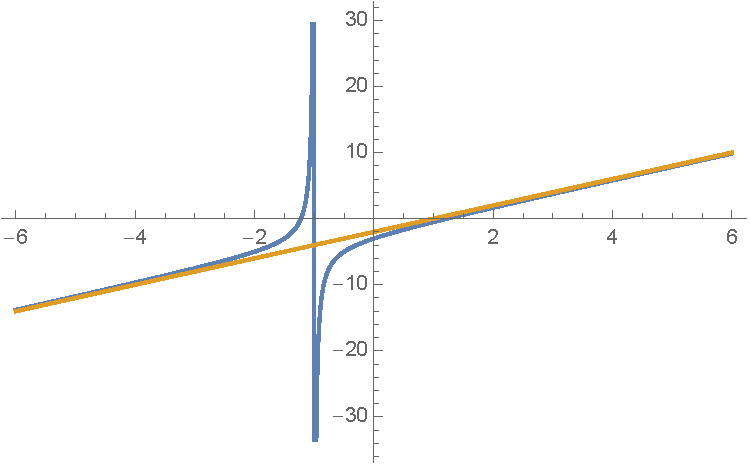
\includegraphics{./images/ch3/asyx.pdf}}
\end{center}

\section{函数的连续性}

\subsection{定义}

{\bf 定义3.4.1:}函数$f(x)$在$x_0$连续:
$$\limx{x_0}f(x)=f(x_0)$$

\begin{itemize}
  \item $f(x)$在$x_0$有定义 
  \item $\limx{x_0}f(x)$存在 
  \item $f(x_0)=f(x_0+0)=f(x_0-0)$
\end{itemize}

{\bf 注:}必要时,可以只考虑函数在某点一侧的连续性,即所谓左(右)连续,
参见教材定义3.4.2-3

{\bf 例:}证明:$f(x)=xD(x)$只在$x=0$处连续。

[提示]:先证明$xD(x)$仅在$x=0$处极限存在。

{\bf 教材3.4.1节-例3:}设$f(x)$在$(-\infty,+\infty)$上有定义,
且对任意$x,y\in (-\infty,+\infty)$,有
$$f(x+y)=f(x)+f(y),$$
则$f(x)$在$(-\infty,+\infty)$上连续,当且仅当$f(x)$在$x=0$连续。

% \begin{center}
% 	\resizebox{!}{4cm}{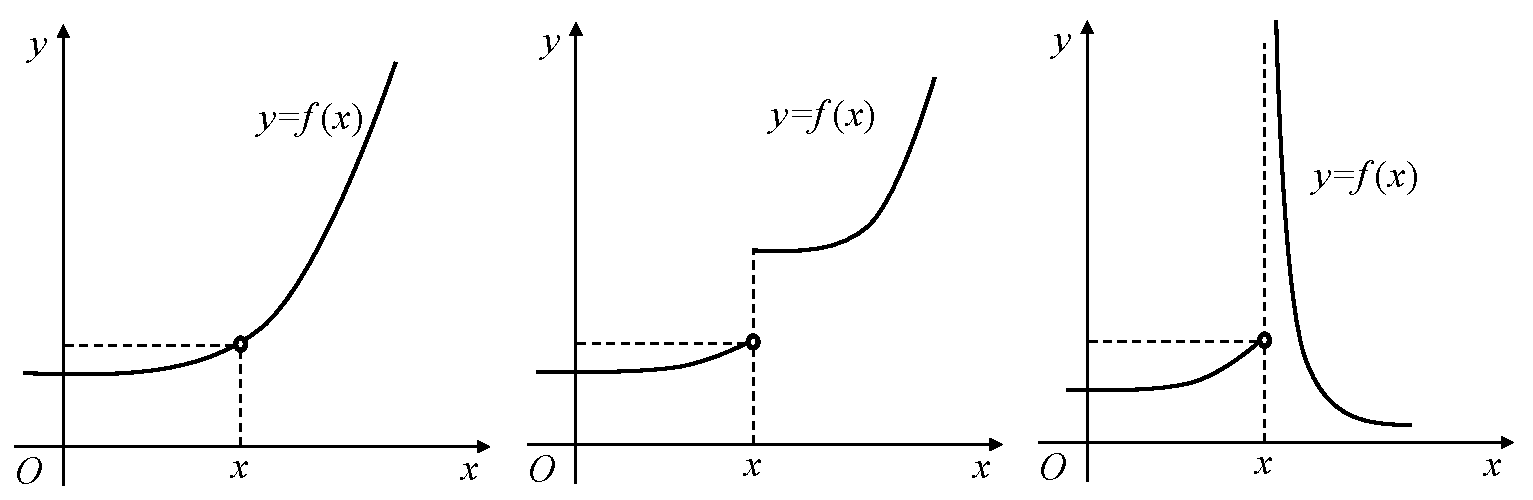
\includegraphics{./images/ch3/notCont.pdf}}
% \end{center}

{\bf 定义3.4.4:}设$x_0$是$f(x)$的间断点(不连续点),对其分类定义如下:
\begin{enumerate}[(1)]
  \setlength{\itemindent}{1cm}
  \item {\bf 第一类间断点:}$f(x_0+0),f(x_0-0)$均存在
  \begin{itemize}
    \item {\it 跳跃间断点:}$f(x_0+0)\ne f(x_0-0)$,例:$y=[x]$当$x$为整数时
    \begin{center}
		\resizebox{!}{4cm}{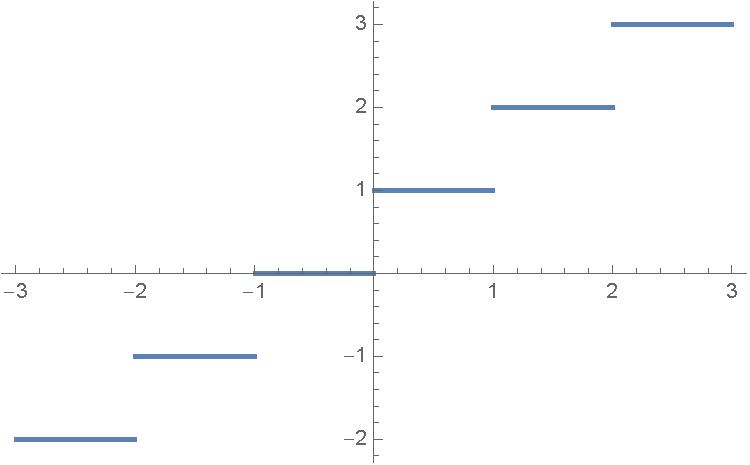
\includegraphics{./images/ch3/roundx.pdf}}
 	\end{center}
    \item {\it 可去间断点:}$f(x_0)$无定义,或
    $$f(x_0)\ne f(x_0+0)=f(x_0-0)$$
    例:$y=\df{\sin x}x$在$x=0$处
    \begin{center}
		\resizebox{!}{4cm}{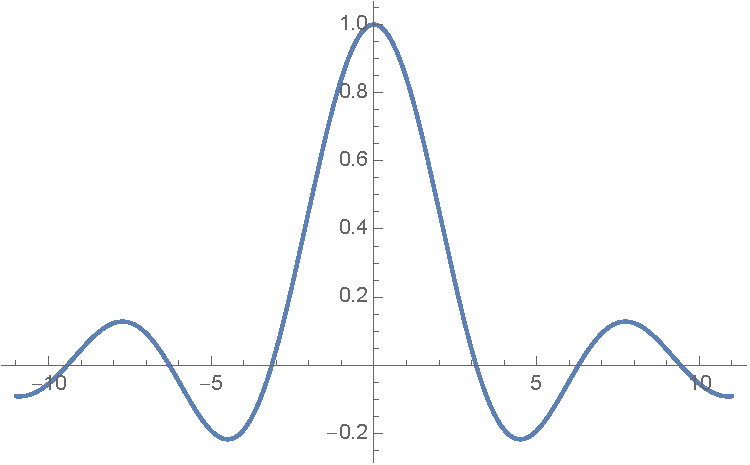
\includegraphics{./images/ch3/sinxox.pdf}}
 	\end{center}
  \end{itemize}
  \item {\bf 第二类间断点:}$f(x_0+0),f(x_0-0)$不同时存在
  \begin{itemize}
    \item {\it 无穷间断点:}某个单侧极限趋于无穷,例:$y=\tan x$和$y=\sec x$在$x=k\pi+\df{\pi}2$处
     \begin{center}
		\resizebox{!}{4cm}{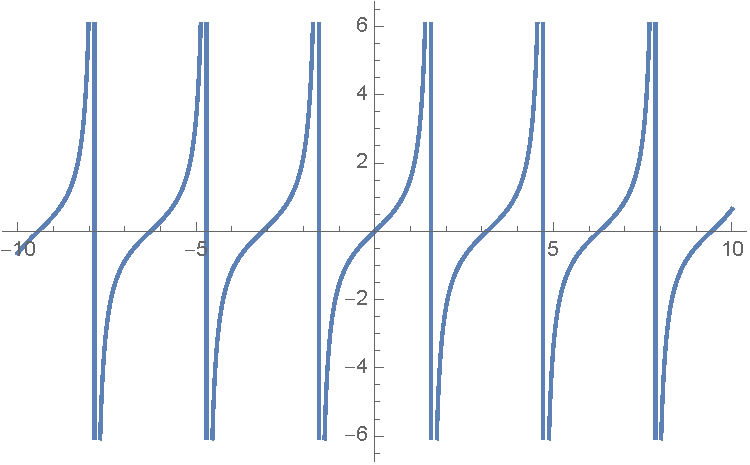
\includegraphics{./images/ch3/tanx.pdf}}
		\resizebox{!}{4cm}{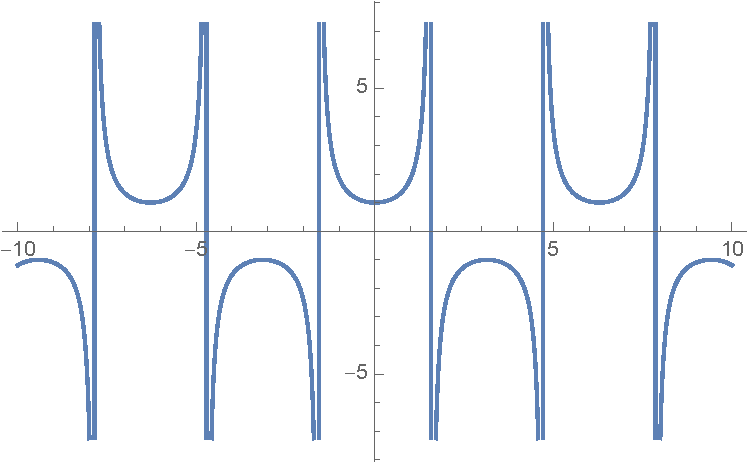
\includegraphics{./images/ch3/secx.pdf}}
 	\end{center}
    \item {\it 振荡间断点:}某个单侧极限不存在,且非无穷,例:$y=\sin\df1x$在$x=0$处
    \begin{center}
		\resizebox{!}{5cm}{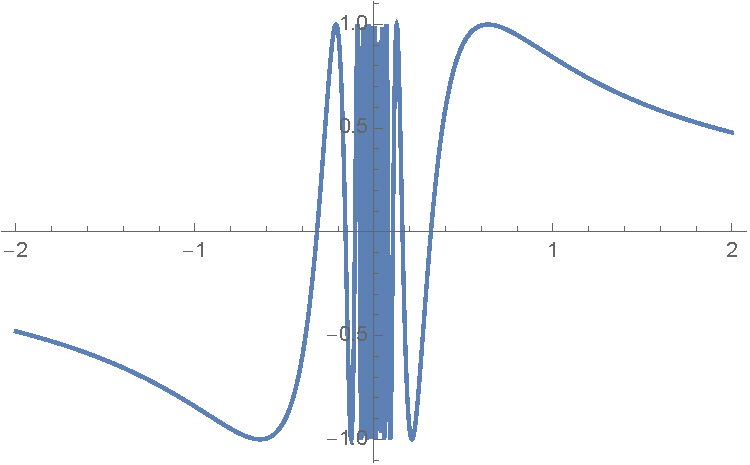
\includegraphics{./images/ch3/sin1ox.pdf}}
 	\end{center}
  \end{itemize}
\end{enumerate}

{\bf 例:}指出以下函数的间断点,判断其类型
\begin{enumerate}[(1)]
  \setlength{\itemindent}{1cm}
  \item $y=\df{x^2-1}{x-1}$\quad{\it 可去}
  \item $y=\df{x^2+1}{x-1}$\quad{\it 无穷}
  \item $y=D(x)$\quad{\it 振荡}
\end{enumerate}

\subsection{基本性质}

{\bf 定理3.4.1-3.4.4:}
\begin{enumerate}[(1)]
  \setlength{\itemindent}{1cm}
  \item {\it 四则运算:} 四则运算仍保持函数的连续性 
  \item {\it 复合函数:} 连续函数的函数运算可以和极限运算交换次序 
  \item {\it 反函数:} 连续函数的反函数也连续 
  \item {\it 初等函数:} 初等函数在其定义域内连续
\end{enumerate}

\subsection{连续函数在有界闭区间上的性质}

\subsubsection{【最值定理】}

{\bf 定理3.4.5:}设$f(x)\in C[a,b]$,则$f(x)$在$[a,b]$上可取到最大和最小值。

{\it 也即,存在$\xi,\eta\in[a,b]$,是对任意$x\in[a,b]$,总有$f(\xi)
\leq f(x)\leq f(\eta)$}

{\bf 推论:}设$f(x)\in C[a,b]$,则$f(x)$在$[a,b]$上有界。

{\bf 例:}设$f(x)\in C[a,+\infty)$,且$\limx{+\infty}f(x)$存在,
证明:$f(x)$在$[a,+\infty)$上有界。

[提示]:首先利用函数极限的有界性证明,存在$M_1$和$X$,对任意$x>X$,有$|f(x)|<M_1$。
然后,利用连续函数在闭区间上的有界性,说明存在$M_2$,对任意$x\in[a,X]$,有$|f(x)|<M_2$。
综合即证。

\subsubsection{【介值定理】}

{\bf 定理3.4.6:}设$f(x)\in C[a,b]$,$M,m$分别为$f(x)$在$[a,b]$上的最大和最小值,
则对任意$\gamma\in[m,M]$,存在\ps{\b “存在”与“至少存在”意义是完全一致的!}
$\xi\in[a,b]$,使得$f(\xi)=\gamma$。

{\bf 推论}(零值定理/零点存在性)
设$f(x)\in C[a,b]$,且$f(a)f(b)<0$,则$f(x)$在$[a,b]$上必有零点。

{\bf 推论'}(零点存在性定理的推广)
\begin{enumerate}[(1)]
  \setlength{\itemindent}{1cm}
  \item {\b 设$f(x)\in C(a,b)$,且$f(a+0)\cdot f(b-0)<0$,则$f(x)$在$(a,b)$内有零点。} 
  \item {\b 设$f(x)\in C(-\infty,+\infty)$,且$f(-\infty)\cdot f(+\infty)<0$,
  则$f(x)$在$(-\infty,+\infty)$内有零点。}
\end{enumerate}

[提示]:利用极限的保号性证明。

{\bf 例:}设$a_0\ne 0$,证明:以下方程至少有一个实根\ps{\b 奇数次多项式方程至少有一个实根!}
$$a_0x^{2n+1}+a_1x^{2n}+\ldots+a_{2n}x+a_{2n+1}=0.$$

[提示]:$\limx{\infty}\df{f(x)}{x^{2n+1}}=a_0$,利用极限保号性说明
$f(x)$当$x$充分大(小)时,分别有取正和取负的值。

{\bf 例:}已知$f(x)\in C[0,3]$,且$f(0)=f(3)$,证明:至少存在
一个$\xi\in[0,2]$,使得$f(\xi+1)=f(\xi)$

{\bf 证:}设$F(x)=f(x+1)-f(x)$,显然$F(x)\in C[0,2]$。

注意到若$f(0)=f(1)$或$f(1)=f(2)$或$f(2)=f(3)$,结论显然成立。故以下设$f(0)\ne f(1),
f(1)\ne f(2),f(2)\ne f(3)$。

不妨设$f(1)>f(0)$,则$F(0)>0$。此时,若$f(2)<f(1)$,则$F(1)<0$,
由连续函数的介值定理可知必有$\xi\in[0,1]$,使得$F(\xi)=0$。
又若$f(2)>f(1)$,则$F(1)>0$,
$$F(2)=f(3)-f(2)=f(0)-f(2)<f(1)-f(2)=-F(1)<0,$$
同样由连续函数的介值定理可知必有$\xi\in[1,2]$,
使得$F(\xi)=0$。

综上,必有$\xi\in[0,2]$,使得$F(\xi)=0$,也即$f(\xi+1)=f(\xi)$。

{\bf 例:}设$G$是第一象限内的一个有界区域(其边界为连续的简单闭曲线),$ABCD$表示
它的一个外接矩形。矩形的一条边与$x$轴的夹角记为$\theta$,如果对于任意$\theta\in
[0,\pi/2]$,$G$总可以被某个外接矩形所围,证明:至少存在某个$\theta_0\in[0,\pi/2]$,
使得与之对应的外接矩形恰好为正方形。({\it 推论:任一平面有界区域都可以内接于某个正方形})

\begin{center}
	\resizebox{!}{6cm}{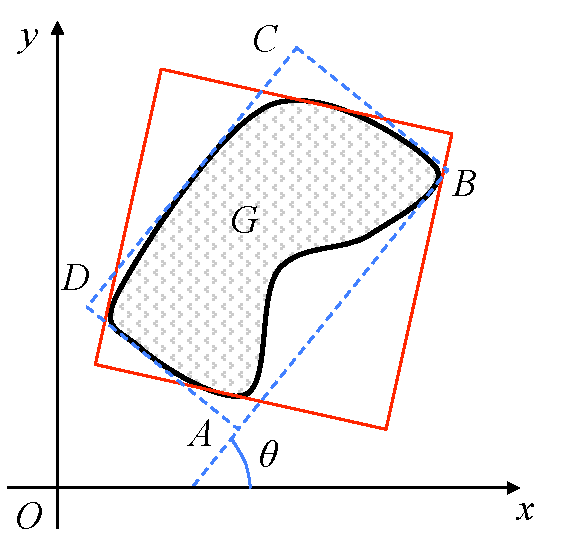
\includegraphics{./images/ch3/sqOut.pdf}}
\end{center}

[提示]:记$l_1(\theta),l_2(\theta)$分别为$AB$和$BC$的长度,显然
$$l_1(0)=l_2(\pi/2),\quad l_2(0)=l_1(\pi/2).$$
令$f(\theta)=l_1(\theta)-l_2(\theta)$,由介值定理可以证明$f(\theta)$存在零点。

{\bf 例:}证明:给定任意平面有界区域,以及一个向量,一定存在一条与该向量平行的直线
平分该区域。

{\bf 例:}证明:给定任意平面有界区域,一定存在两条相互垂直的直线,将其四等分。

[提示]:设其中一条直线的极角为$\theta$,则另一条的为$\theta+\pi/2$。
分别记两条直线为$l_{\theta}$和$l_{\theta+\pi/2}$,显然可以使得二者都平分给定区域。
设此时四个区域的面积按顺时针方向依次为$S_1,S_2,S_3,S_4$,且由平分可满足
$$A_1+A_2=A_3+A_4,\quad A_1+A_4=A2+A_3,$$

\begin{center}
	\resizebox{!}{6cm}{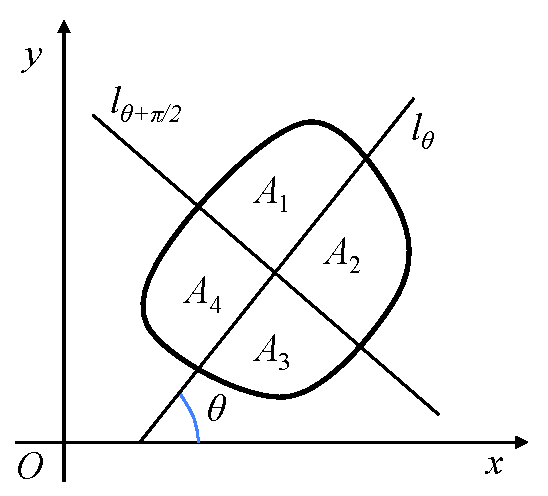
\includegraphics{./images/ch3/4cut.pdf}}
\end{center}

由此可得
$$A_1=A_3,\quad A_2=A_4.$$
进而,只需适当取$\theta$,使得$A_1=A_2$即可。

记$f(\theta)=A_1(\theta)-A_2(\theta)$,不妨设$f(0)>0$,从而
$$f(\pi/2)=A_1(\pi/2)-A_2(\pi/2)=A_4(0)-A_1(0)=A_2(0)-A_1(0)=-f(0)<0,$$
由介值定理,即证。

{\bf 例:}任意金属圆环上,总存在相对的两点温度相同。
({\it 圆环可以看成赤道,温度即为两点的气温})

[提示]:默认假设温度总是连续分布的。

{\bf 思考:}构造更多类似的例题,用介值定理证明某种状态的存在性。

\newpage

% \section*{补充例题}
% \addcontentsline{toc}{section}{补充例题}
% 
% {\bf 例}:证明函数$f(x)=\left\{\begin{array}{ll}
% x,\;&x\in\mathbb{Q}\\ 0,\;&\mathrm{else}
% \end{array}\right.$
% 仅在$x=0$连续
% 
% {\bf 证:}显然$f(0)=0$。注意到
% $$0<|f(x)|\leq |x|,$$
% 而$\lim\limits_{x\to 0}|x|=0$,故由夹逼定理
% $$\lim\limits_{x\to 0}f(x)=0=f(0),$$
% 也即$f(x)$在$x=0$连续。
% 
% \bigskip
% 
% 设$x_0\ne 0$,下证$\lim\limits_{x\to x_0}f(x)$不存在,进而可知
% $f(x)$在$x_0$处不连续。事实上,若设$\lim\limits_{x\to x_0}f(x)$存在,
% 则
% $$\lim\limits_{x\to x_0}D(x)=\frac{\lim\limits_{x\to x_0}f(x)}
% {\lim\limits_{x\to x_0}x}$$
% 也存在,从而与$D(x)$在任意点处极限不存在矛盾。
% 
% 综上,$f(x)$仅在$x=0$连续。
% 
% \newpage
% 
% \newpage

\section*{课后作业}
\addcontentsline{toc}{section}{课后作业}

{\bf 【必作题】}

\begin{itemize}
  \item 习题3.1:4(1,3),7,15
  \item 习题3.2:2,3,4,5
  \item 习题3.3:2,4,5,7(2,6),8,9,10(3,4)
  \item 习题3.4:5(1-3),9,15,17
\end{itemize}

\bigskip

\hrule

\bigskip
\bigskip

{\bf 【思考题】}
\begin{itemize}
  \item 习题3.1:10,11,12
  \item 习题3.2:6,7
  \item 证明:$$\limn\left\{\lim\limits_{m\to\infty}\left[\cos^{2m}(n!\pi
	x)\right]\right\}=D(x)$$
	其中$D(x)$为Dirichlet函数
%   \item 自学3.3.3节:渐近线 
  \item 习题3.3:1,6,12,13
  \item  计算极限
	\begin{enumerate}[(1)]
% 	  \setlength{\itemindent}{1cm}
	  \item $\limx{+\infty}(\sqrt{x^2+x+1}-\sqrt{x^2+x-1})$ 
	  \item $\limx{0}\df{\sqrt[3]{1+x}-1}{x}$ 
	  \item $\limx{0}\df{\sqrt{1-\cos x^2}}{1-\cos x}$ 
	  \item $\limx{0}\df{1-\cos x\cos 2x}{1-\cos x}$
	  \item $\limx{\pi /4}(\tan x)^{\tan 2x}$ 
	  \item $\limx{0}\left(2e^{\frac{x}{x+1}}-1\right)^{\frac{x^2+1}{x}}$ 
	  \item $\limx{+\infty}\left(\sqrt{x^2+x}-\sqrt[3]{x^3+x^2}\right)
% 	  =
% 	  \limx{+\infty}x\left(1+\df1x\right)^{\df13}\left[\left(
% 	  1+\df1x\right)^{\df16}-1\right]=\df16
		$ 
	  \item $\limx{+\infty}\left(\df{x^2-1}{x^2+1}\right)^{x^2}$
	  \item $\limx{0}\left(\df{a^x+b^x+c^x}{3}\right)^{1/x}\,(a,b,c>0)$ 
	  \item $\limx{0}\left(\df{a^{x+1}+b^{x+1}+c^{x+1}}{a+b+c}\right)^{1/x}
	  \,(a,b,c>0)$ 
	  \item $\limx{0}\df{\tan(\tan x)-\sin(\sin x)}{\tan x-\sin x}$
	\end{enumerate}
  \item 习题3.4:1,3,13,14,16,19
  \item 设$a_1<a_2<\ldots<a_n$,证明以下方程有$n-1$个实根
	$$\df 1{x-a_1}+\df 1{x-a_2}+\ldots+\df 1{x-a_n}=0.$$
\end{itemize}

\newpage

% {\Large\it

% }